%%%%%%%%%%%%%%%%%%%%%%%%%%%%%%%%%%%%%%%%%
% Simple Sectioned Essay Template
% LaTeX Template
%
% This template has been downloaded from:
% http://www.latextemplates.com
%
% Note:
% The \lipsum[#] commands throughout this template generate dummy text
% to fill the template out. These commands should all be removed when 
% writing essay content.
%
%%%%%%%%%%%%%%%%%%%%%%%%%%%%%%%%%%%%%%%%%

%----------------------------------------------------------------------------------------
%	PACKAGES AND OTHER DOCUMENT CONFIGURATIONS
%----------------------------------------------------------------------------------------

\documentclass[12pt]{article} % Default font size is 12pt, it can be changed here

\usepackage{synttree}
\usepackage{longtable}
\usepackage{geometry} % Required to change the page size to A4

\geometry{a4paper} % Set the page size to be A4 as opposed to the default US Letter

\usepackage{graphicx} % Required for including pictures

\usepackage{float} % Allows putting an [H] in \begin{figure} to specify the exact location of the figure
\usepackage{wrapfig} % Allows in-line images such as the example fish picture

\usepackage{lipsum} % Used for inserting dummy 'Lorem ipsum' text into the template

\linespread{1.2} % Line spacing

%\setlength\parindent{0pt} % Uncomment to remove all indentation from paragraphs

\graphicspath{{./Pictures/}} % Specifies the directory where pictures are stored

\begin{document}

%----------------------------------------------------------------------------------------
%	TITLE PAGE
%----------------------------------------------------------------------------------------

\begin{titlepage}

\newcommand{\HRule}{\rule{\linewidth}{0.5mm}} % Defines a new command for the horizontal lines, change thickness here

\center % Center everything on the page

\textsc{\LARGE University of Glasgow}\\[1.5cm] % Name of your university/college
\textsc{\Large Safety Critical Systems 4}\\[0.5cm] % Major heading such as course name

\HRule \\[0.4cm]
{ \huge \bfseries Safety Analysis Tool\\ for a Formula 1 Race }\\[0.4cm] % Title of your document
\HRule \\[1.5cm]

\begin{minipage}{0.4\textwidth}
\begin{flushleft} \large
\emph{Author:}\\
Garry \textsc{Sharp}\\ % Your name
\textsc{0801585s}
\end{flushleft}
\end{minipage}
~
\begin{minipage}{0.4\textwidth}
\begin{flushright} \large
\emph{Course Co-Ordinator:} \\
Dr. Chris \textsc{Johnson} % Supervisor's Name
\end{flushright}
\end{minipage}\\[4cm]

{\large 19th of November 2012}\\[3cm] % Date, change the \today to a set date if you want to be precise

%\includegraphics{Logo}\\[1cm] % Include a department/university logo - this will require the graphicx package

\vfill % Fill the rest of the page with whitespace

\end{titlepage}

%---
% Prelude
%----

\begin{abstract}

Formula 1 has always been a sport in which tragedy has had the misfortune to echo throughout its history. The often fervent debate surrounding the sport's safety has lead to much increased safety standards within the past 30 years as there has not been a death in the sport for many years now (although there have been recent deaths in similar sports MotoGP and Indy 500). However, the sport transitioning into a new era has brought about new threats and concerns to both drivers and members of the public. A good example of this could be the terrorist threats this year in advance of the Bahrain GP.

After the infamous death of Aryton Senna in Imola on the 1st of May 1994 (and Roland Ratzenberger in qualifying the day before), many pioneered for increased standards within the sport. Although the actual rate of innovation in safety after this did not increase at all. Innovations continued to be made before the deaths of Senna and Ratzenberger (such as mandatory fire proof clothing for all pit crew and the introduction of a safety car after crashes).

This tool aims to objectively quantify the risks involved at any specific race by accepting an array of conditions as an input and then contrasting the likelihood of these conditions to occur and cause an accident with that of the presumed and generally accepted effectiveness of the measures designed to counteract them. The focal point of safety will be on that of the drivers, although, there will invariably be some cross over with other people included in a formula 1 event, this will be especially highlighted when this impacts on the driver in some way.

\end{abstract}

\newpage

%----------------------------------------------------------------------------------------
%	TABLE OF CONTENTS
%----------------------------------------------------------------------------------------

\tableofcontents % Include a table of contents

\newpage % Begins the essay on a new page instead of on the same page as the table of contents 

%----------------------------------------------------------------------------------------
%	Safety in Foruma 1
%----------------------------------------------------------------------------------------

\section{Introduction to Safety in Formula 1} % Major section

We will examine what has happened in previous Formula 1 events, the consequences of some of these events as well as
continuing innovations in safety in the sport. The governing body of Formula 1 is the FIA (Federation Internationale de l'Automobile), who are a very well known name in Formula 1 and all motorsport throughout the world. The responsibility of the safety of the drivers and other members of the Formula 1 team is their responsibility. Nowadays, and all of their regulations for the current season can be found on their website\\

%------------------------------------------------

\subsection{Summary of Previous Diasters} % Sub-section

Formula 1 has had the misfortune of being littered with disastrous past events, a look at a list of fatalities illustrates how fierce the sport can be (see appendix A). It should be noted that in modern Formula 1 events, safety is something that is taken very seriously. The FIA have an ever expanding list of regulations to ensure that the safety of their events is the best it can be.

%------------------------------------------------

\subsection{Preventative Measures Taken} % Sub-section
There have been many past attempts to make Formula 1 100\% safe. Some examples include the addition of a track safety car, gravel traps to slow the cars as well as permentent medical centres being compulsory at all Formula 1 tracks. There were, of course, always people to push the changes through. Jackie Stewart, a now retired Formula 1 driver was considered the ambassador of safety for the sport. He first became concerned with the safety of the sport after a crash in the Spa Grand Prix when he became trapped under his car after a crash. After a long wait for an ambulance to arrive, he then had to endure a long and arduous trip to the hospital where, of course, the ambulance got lost en route. Luckily he was not seriously injured. The shock statistic of the time, he claims, was that people racing during his era had a roughly a two in three chance of dying. The last death in the sport was that of Aryton Senna in 1994, and since then the FIA have endeavoured to ensure that safety remains paramount in Formula 1 safety. Attached in the references is a history of all the major safety changes made throughout the seventies, eighties and nineties.

%------------------------------------------------


%----------------------------------------------------------------------------------------
%	MAJOR SECTION 1
%----------------------------------------------------------------------------------------

\section{Safety Analysis} % Major section

Any seasoned formula 1 fan will tell you that no two races are ever the same, this of course is true for many sporting events, however, where formula 1 (and motorsport in general) differ is that each driver is in command of a machine that can cause immense damage to other drivers.

%------------------------------------------------

\subsection{Tool Description}

I've elected to use a technique based upon the FMECA technique in the development of the tool, the tool will examine a series of failure modes and after entering certain values, output to a risk matrix the detectability vs severity of that particular failure mode. The tool also displays in the top right hand corner the RPN based on the occurance rate which is also calculated for each failure mode (but not reflected in the risk matrix). The values required to calculate the RPN (The severity, occurrence and detection rates) will be calculated based on  user input. There will also be a slight amount of cross over between failure modes (for instance if one of the Electronica Control Units or ECUs breaks in a formula 1 car, then the chances of being forewarned of catastrophic engine failure is drastically reduced), unfortunately, this is not reflected in the implementation, although, it is highlighted for each failure mode.

\subsection{Block Diagrams}

Block diagrams are a very good tool for determining the weak aspects of a system that may be instrumatal in realising a failure mode. However, for the tool that I have developed I decided to omit the diagrams as I felt that the tool is too general to make any substantial gains from the inclusion of the diagrams. In my evaluation section, I discuss the concept of further development of the system to include more failure modes and better numerical analysis in determining the RPN. Should the failure modes be further developed. In this scenario when trying to identify ALL of the safety concerns and failure modes, the usage of block diagrams would aid greatly, however, as I am merely trying to encapsulate a broader spectrum of the main failure modes, the usage of block diagrams seems inapproapriate.

\subsection{Failure modes}

Please refer to the appendices to see a full list of Failure Modes and Effects that have been incorporated into the tool.

\subsection{Unpredictable Events \& Human Factors} % Sub-section


\begin{wrapfigure}{l}{0.50\textwidth} % Inline image example
  \begin{center}
    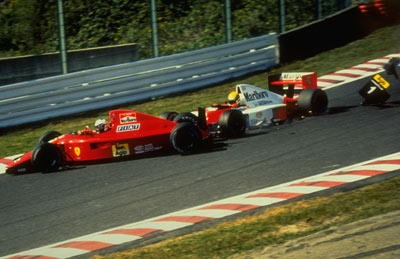
\includegraphics[width=0.45\textwidth]{senna-prost}
  \end{center}
\parbox{7cm}{\caption{Aryton Senna deliberately runs Alain Prost off the track at Suzuka in the 1990 Japan Grand Prix}}
\end{wrapfigure}

It is not always the case in Formula 1 events that the drivers necessarily reflect the risks involved in their racing style. Even after performing a thorough risk assessment (FMECA or otherwise), should a driver or a member of the public exercise a pre-mediated stunt (or simply do something entirely stupid) then there are only certain provisions that can be put in place to handle the resulting events. Figure 2 famously shows Aryton Senna crashing into Alain Prost after feeling cheated that he did not start on the correct side of the track. Although neither driver was injured and safety provisions had been put in place, other than the FIA changing the grid block positions, there is not a lot that they could have done to have prevented the crash. This level of recklessness is not uncommon in formula 1. Indeed a false start by Romain Grojean at Spa this season created a similar crash where he instantly caused three cars (including his own) to be retired straight away. The FIA punished him accordingly and he received a race ban. Essentially, this demonstrates that the hazards captured by FMECA or any other risk assessment technique, are subject to random events which cannot accurately be predicted.

%------------------------------------------------

%------------------------------------------------

\subsection{Further Information} % Sub-sub-section
\subsubsection{Team Responsibility}
In addition to the regulations that the FIA impose, each of the teams is expected to perform their own safety analysis and fully test their cars before driving, this, however, does not always mean that the vehicle is safe. For instance, this season Lewis Hamilton's McLaren MP4-27 broke unexpectedly 3 times causing him to retire from the races. It is, therefore, very important to understand that despite extensive testing from teams, that there is still (an albeit reduced) risk of unexpected failure.
%----------------------------------------------------------------------------------------
%	EVALUATION
%----------------------------------------------------------------------------------------

\section{Evaluation}

Due to the scale and nature of Formula 1 events, it would be extremely difficult to do any practical testing of the system. That does not, however, mean that general testing regarding the method and techniques cannot be performed. A reasonable way of going about the evaluation of the system would be to compare and contrast it to existing systems, and by careful examination of results, make a conclusion based on the accuracy of the system. It should be noted that initial sanity testing against a similar system resulted in a significant change of code, meaning that the version submitted is actually version 3 (with two major re-writes prior to this version), this means that some of the changes made in this system will not be obvious from looking at the tool in its current state.

\subsubsection{The bathtub failure model}
There are restrictions placed on the number of cars, engines and gearboxes that each driver may use, this can have an impact on the stability of the car. Each team is allowed no more than two cars at a time and should a new car be used between qualifying and the race, the driver of that car will start the race from the pit lane. Each driver is allowed at most eight engines per season and one gearbox per five races. The bathtub failure model (also known as the bathtub curve) is a model that explains the failure rate of hardware as a function of time illustrating that there is a high failure rate at the start of usage (known as the break in phase) and also towards the end of its life (known as the wear out phase). The tool that has been developed does not account for the changes in gearboxes or engines during the season due to time constraints.

\begin{center}
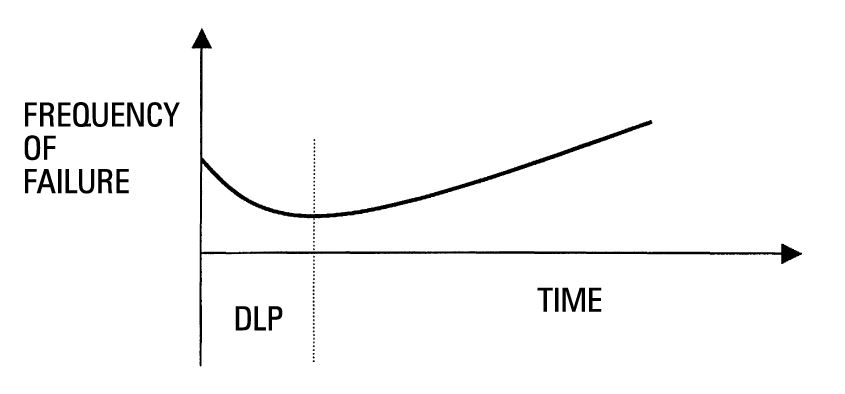
\includegraphics[width=0.7\linewidth]{bathtub}
\parbox{10cm}{\caption{Bathtub model showing hardware life cycle as a function of time}}
\end{center}

\subsubsection{Significant Changes to the System}

After the initial implementation (along with basic sanity testing and comparison to a peer's model) it became apparent that a few things needed to be drastically changed, some of these changes can be documented below
\begin{center}
\begin{tabular}{p{3cm} p{10cm}}
Previous Item & Revision \\
\hline \\
Interface \& Interactivity & My initial system had been entirely paper based, it basically operated in a traditional paper based FMECA manner (a simple worksheet). I very quickly realised that making the system more interactive would allow for better, more personalised feedback to be given. I therefore started on a simple HTML mockup of the worksheet. This later changed again to be reflected in a risk matrix. \\
Criticality Analysis & The initial system also did not feature any criticality analysis (this was mostly so that I could see what a more basic mock up of the system would look like before adding functionality), the addition of the criticality analysis feature was not something that I considered would pose that much more of a problem given the scope that I was working in, this was the major inspiration behind the development of the risk matrix. \\
Local RPN & Initially, the plan was simply to output in each case to the risk martix. The problem with this is that the risk matrix only compares the detectability and the severity, which does not reflect the true RPN of the failure mode as it does not take into account the occurance rate. This was implemented to be shown at the same time as a value is added to the risk matrix.
\end{tabular}
\end{center}

\subsubsection{User evaluation}

To see if the outputted values to my risk matrix were correct I did an informal evaluation of the system (I opted for the informal technique as any major findings from this would not make a big difference to the system. ie factor values in the RPN engine would change a small amount). The evaluation took the form of giving paper risk matrices to peers and asking them to make an educated guess as to where to plot the probability against the severity given a condition for a failure mode (eg if stewards are present in the event of a terrorist attack). Surprisingly, the answers I received were close to my own which suggests that the values that I guessed using intuition \& the values I researched were close to what others would naturally guess they were. I still believe though that the system would benefit greatly with regards to validy should real statistics be used.

\subsubsection{Effectiveness of the Tool}

The tool in general seems to function as desired (basic black box testing showed that it output the correct values when given an input certain input set). What still remains unclear is how well the system would function should it be employed in the safety critical analysis of a Formula 1 event. As this system focusses on the broader idea of Formula 1 driver safety and not a particular aspect of it, it has been very difficult to go into detail that, in a real race, would be sufficient enough to perform a serious and accurate test. The current list of FIA regulations spans many pages, with each racing team adhering to these instructions as well as taking their own safety precautions. Although my tool addresses a subset of each of the safety aspects of a formula 1 race (spectator positioning, pit lane procedures, racing maneuvers etc), it does not go as deep as to asses the criticality of each FIA regulation, and as such, cannot possibly claim to be more substantial than the already existing system. That said, in terms of providing a summary (which could be used when presenting a general and overall danger at an event) I would claim that my tool is quite effective. I think its greatest strength is when used in conjunction with another tool or the general regulatory FIA risk assessment, but not as the primary tool in safety analysis.

Another factor to consider is that lots of the numbers used to generate the RPNs are constructed using intuition and research where available. For instance, it would be very logical to presume that the detectability of a brake failure would be more likely should the brakes be checked before the race. However, as a system which attempts to output quantitative data, it is very difficult to say indefinitely that this increases the detectability by a factor of x. As a fan of Formula 1 I have used values (where applicable) that I believe to be close to what the actual values would be. This means that any RPN that is output to the risk matrix is not entirely accurate, rather, an approximation of the likelihood of an event against its detectability.


%Highlight that it would never realistically get used. FIA are a v.large and responsible organisation. Safety in F1 has already increased significantly

%----------------------------------------------------------------------------------------
%	Findings & Conclusions
%----------------------------------------------------------------------------------------

\section{Findings and Conclusions}
\subsection{Further Development}
In my opinion, there are two ways in which the system can be made to be more accurate. Firstly, the inclusion of more failure modes would allow for more in-depth analysis and would almost certainly highlight new safety concerns. Secondly the addition of real statistical data in the RPN engine would make the values calculated much more accurate. Due to time constraints, mining this data proved insurmountable to the functioning of the system, so intuitive values were used.
\subsection{Conclusive Summary}
Overall, testers found that the system does a good job of illustrating the safety concerns of a Formula 1 race along with providing insight as to how performing certain actions or adding certain failsafe measures, can mitigate the risks. In this regard they system is a complete success (see above for how it could be further improved). However, I do not feel that by today's strict Formula 1 standards, that my tool would aid organisers of an event. Whilst researching safety and safety history in Formula 1. Whilst investigating Formula 1 safety it became abundantly apparent that there is already a lot of money involved in keeping the sport safe. I do feel that the tool could eventually provide useful feelback and analysis, but only afer the steps detailed above in the further development stage have been performed.
%----------------------------------------------------------------------------------------
%	BIBLIOGRAPHY
%----------------------------------------------------------------------------------------
\newpage
\begin{thebibliography}{99} % Bibliography - this is intentionally simple in this template

\bibitem
\newblock "About FIA". Fédération Internationale de l'Automobile (FIA). Viewed 19 Nov 2012.\\ http://www.fia.com/en-GB/the-fia/about-fia/Pages/AboutFIA.aspx
\bibitem
\newblock  Formula 1/FIA. "The seventies". Retrieved 19 Nov 2012.\\ http://www.formula1.com/inside\_f1/safety/a\_history\_of\_safety\_in\_formula\_one/7425.html
\bibitem
\newblock  Formula 1/FIA. "The eighties". Retrieved 19 Nov 2012.\\ http://www.formula1.com/inside\_f1/safety/a\_history\_of\_safety\_in\_formula\_one/7426.html
\bibitem
\newblock  Formula 1/FIA. "The nineties". Retrieved 19 Nov 2012. \\http://www.formula1.com/inside\_f1/safety/a\_history\_of\_safety\_in\_formula\_one/7427.html
\bibitem
\newblock Williamson, Martin. "A Brief History of Formula One". ESPN. Viewed 19 Nov 2012. \\http://en.espnf1.com/f1/motorsport/story/3831.html
\bibitem
\newblock FIA. Official Website. Accessed 19 Nov 2012.\\ http://www.fia.com/en-GB/Pages/HomePage.aspx
\bibitem 
\newblock FIA. FIA 2012 technical regulations. Accessed 19 Nov 2012.\\ http://www.fia.com/en-GB/sport/regulations/Pages/FIAFormulaOneWorldChampionship.aspx
\bibitem 
\newblock FIA. FIA 2012 sporting regulations. Accessed 19 Nov 2012.\\ http://www.fia.com/en-GB/sport/regulations/Pages/FIAFormulaOneWorldChampionship.aspx
\bibitem
\newblock FIA. FIA Standards List. Various items listed, accessed from 12 Nov - 19 Nov 2012.\\ http://www.fia.com/en-GB/sport/regulations/Pages/FIAStandards.aspx
\bibitem
\newblock FIA. Hall of Fame (Jackie Stewart). accessed 19 Nov 2012.\\ http://www.formula1.com/teams_and_drivers/hall_of_fame/127/
\bibitem
\newblock Dennis J. Wilkins. The bathtub curve. accessed 19 Nov 2012 \\ http://www.weibull.com/hotwire/issue21/hottopics21.htm
 

\end{thebibliography}
\newpage
\appendix
\section{Formula 1 Deaths}
\begin{center}
\begin{longtable}{p{8cm} p{4cm}}
Name & Date of Death \\
\hline \\
Cameron Earl (UK)&June 18, 1952 \\
 Chet Miller (USA)&May 15, 1953\\
 Charles de Tornaco (BEL)&September 18, 1953\\
 Onofre Marimón (ARG)&July 31, 1954\\
 Mario Alborghetti (ITA)&April 11, 1955\\
 Manny Ayulo (USA)&May 16, 1955\\
 Bill Vukovich (USA)&May 30, 1955\\
 Eugenio Castellotti (ITA)&March 14, 1957\\
 Keith Andrews (USA)&May 15, 1957\\
 Pat O'Connor (USA)&May 30, 1958\\
 Luigi Musso (ITA)&July 6, 1958\\
 Peter Collins (UK)&August 3, 1958\\
 Stuart Lewis-Evans (UK)&September 19, 1958\\
 Jerry Unser, Jr. (USA)&May 17, 1959\\
 Bob Cortner (USA)&May 19, 1959\\
 Harry Schell (USA)&May 13, 1960\\
 Chris Bristow (UK)&June 19, 1960\\
 Alan Stacey (UK)&June 19, 1960\\
 Shane Summers (UK)&June 1, 1961\\
 Giulio Cabianca (ITA)&June 15, 1961\\
 Wolfgang von Trips (GER)&September 10, 1961\\
 Ricardo Rodríguez (MEX)&November 1, 1962\\
 Gary Hocking (Rhodesia and Nyasaland)&December 21, 1962\\
 Carel Godin de Beaufort (NED)&August 2, 1964\\
 John Taylor (UK)[C]&August 7, 1966\\
 Lorenzo Bandini (ITA)[D]&May 7, 1967\\
 Bob Anderson (UK)&August 14, 1967\\
 Jo Schlesser (FRA)&July 7, 1968\\
 Gerhard Mitter (GER)&August 2, 1969\\
 Martin Brain (UK)&May 25, 1970\\
 Piers Courage (UK)&June 7, 1970\\
 Jochen Rindt (AUT)&September 5, 1970\\
 Jo Siffert (SUI)&October 24, 1971\\
 Roger Williamson (UK)&July 29, 1973\\
 François Cevert (FRA)&October 6, 1973\\
 Peter Revson (USA)&March 30, 1974\\
 Helmuth Koinigg (AUT)&October 6, 1974\\
 Mark Donohue (USA)&August 19, 1975\\
 Tom Pryce (UK)[E]&March 5, 1977\\
 Brian McGuire (AUS)&August 29, 1977\\
 Ronnie Peterson (SWE)[F]&September 10, 1978\\
 Patrick Depailler (FRA)&August 1, 1980\\
 Gilles Villeneuve (CAN)&May 8, 1982\\
 Riccardo Paletti (ITA)&June 13, 1982\\
 Elio de Angelis (ITA)&May 15, 1986\\
 Roland Ratzenberger (AUT)&April 30, 1994\\
 Ayrton Senna (BRA)&May 1, 1994\\
 John Dawson-Damer (UK)&June 24, 2000\\
 Fritz Glatz (AUT)&July 14, 2002\\
\end{longtable}
\end{center}

%----------------------------------------------------------------------------------------

\end{document}